\section{Napisz program, który wyznaczy epsilon maszynowe dla typu float i double w języku C oraz float w Python przy pomocy programu rekurencyjnego.
}

\paragraph{Kod w C++:}

\begin{minted}{C++}
	#include<iostream>

	using namespace std;


	float epsilon(float curr){
		if(1.0f + curr/2 != 1.0f){
			return epsilon(curr/2);
		}
		else return curr;
	}


	double epsilon(double curr){
		if(1.0 + curr/2 != 1.0){
			return epsilon(curr/2);
		}
		else return curr;
	}

	int main(){
		cout << "epsilon dla floata: " << epsilon(1.0f) << endl;
		cout << "epsilon dla double'a: " << epsilon(1.0) << endl;

	}
\end{minted}


Wyniki programu:

\begin{lstlisting}
epsilon dla floata: 1.19209e-07
epsilon dla double: 2.22045e-16
\end{lstlisting}


Wartości zgadzają się z wartościami na wikipedii. Zaobserwowano, że w zależności od tego czy dodajemy czy odejmujemy od jedynki epsilon różni sie o rzęd wielkości w systemie dwójkowym.
\clearpage
\newpage
\paragraph{Kod w Pythonie:}

\begin{minted}{Python}
	
	def epsilon(curr:float):
		if(1.0 + curr/2 != 1.0):
			return epsilon(curr/2)
		else: 
		return curr
	
	print("Epsilon floata: ", epsilon(1.0))
\end{minted}

Wyniki programu:

\begin{lstlisting}
Epsilon floata:  2.220446049250313e-16
\end{lstlisting}

Wynik jest tożsamy z wynikiem dla double'a w C++, co może wskazywać, że float w Pythonie to liczba zmiennoprzecinkowa o podwójnej precyzji. Po sprawdzeniu w dokumentacji Pythona okazyje się, że rzecywiście tak jest.

\clearpage
\newpage
\section{Napisz dwa programy w języku C bądź Python, gdzie pierwszy zachowuje się niestabilnie i wyjaśnij dlaczego, podczas gdy drugi zachowuje się stabilnie i jest ulepszoną wersją pierwszego programu.
}

Jako przykład wybrano algorytm obliczania wartości funkcji $e^x$ z jej rozwinięcia w szereg Taylora:

$$
e^x = \sum_{n = 0}^\infty {\frac{x^n}{n!}}
$$



Pierwszym naiwnym sposobem jest próba liczenia sumy po prostu poprzez sumowanie wyrazów w pętli:

\begin{minted}{Python}
	def exp(x:int, acc: int):
    	res = 0
    	for i in range (0, acc):
       		res += (x**i)/fact(i)

    return res
\end{minted}

Rozwiązanie to prowadzi do dużych rozbieżności dla $x<0$.  Dzieje się tak, gdyż zadzodzi zjawisko zwane \textit{Catastrophic cancellation}. Polega ono na utracie bitów przy odejmowaniu bardzo bliskich sobie liczb.

Rozwiązaniem problemu jest skorzystanie z faktu, że $e^{-x} = \frac{1}{e^x}$. Oto poprawiony algorytm:

\begin{minted}{Python}

	def bttrexp(x:int, acc: int):
	res = 0
	if x < 0: return (1/bttrexp(-x, acc))
	for i in range (0, acc):
		res += (x**i)/fact(i)
		
	return res
	
\end{minted}
\newpage

Oto cały kod programu:

\begin{minted}{Python}
		
	import math

	def fact(x :int):
		return 1 if x == 0 else fact(x-1)*x
	
	def exp(x:int, acc: int):
		res = 0
		for i in range (0, acc):
			res += (x**i)/fact(i)
	
		return res
	
	def bttrexp(x:int, acc: int):
		res = 0
		if x < 0: return (1/bttrexp(-x, acc))
		for i in range (0, acc):
			res += (x**i)/fact(i)
	
		return res
	
	print("Gorsze: ", exp(-30, 300), "Lepsze: ", bttrexp(-30, 300), "Z biblioteki math: ", math.exp(-30))
	
\end{minted}

Dla zadanych wartości otrzymujemy wynik
\begin{lstlisting}
	Gorsze:  -8.553016433669241e-05 Lepsze:  9.357622968840171e-14 Z biblioteki math:  9.357622968840175e-14
\end{lstlisting}
Jak widać wynik naiwnego algorytmu odbiega od rzeczywistości w przeciwieństwie do poprawionej wersji.

\section{Sumowanie liczb pojedynczej precyzji w języku C:
}
\subsection{Napisz program, który oblicza sumę N liczb pojedynczej precyzji przechowywanych w tablicy o N= $10^7$ elementach. Tablica wypełniona jest tą samą wartością v z przedziału [0.1,0.9] np.v= 0.53125. Zaproponuj dwa takie v, gdzie błędy będą najmniejsze i największe w czasie sumowania.}

\begin{itemize}
	\item Napisz program, który oblicza sumę N liczb pojedynczej precyzji przechowywanych w tablicy o $N= 10^7$ elementach. Tablica wypełniona jest tą samą wartością v z przedziału [0.1,0.9] np.v= 0.53125. Zaproponuj dwa takie v, gdzie błędy będą najmniejsze i największe w czasie sumowania.
	\item Wyznacz bezwzględny i względny błąd obliczeń. Dlaczego błąd względny jest tak duży?
	\item W jaki sposób rośnie błąd względny w trakcie sumowania? Przedstaw wykres (raportuj wartość błędu co 25000 kroków) i dokonaj jego interpretacji.

\end{itemize}

Kod programu:

\begin{minted}{C++}
	#include<iostream>
	#include<iomanip>
	#include<ctime>
	#define e7 10000000
	#define C 0.3728
	using namespace std;

	float normal_sum();


	float *tab;
	int main(){
		cout << setprecision(12);
		clock_t start, end;

		tab = new float[e7];
		for(int i = 0; i < e7; i++) tab[i] = C;

		start = clock();
		float sum = normal_sum();
		end = clock();
		cout << "\nNormal adding time elapsed: " << (end-start)*1.0/CLOCKS_PER_SEC << " ===========";
		cout << "\nSUM/ERROR/RERROR  " <<sum<<" "<< (e7*C - sum) <<" " << (e7*C - sum)/(C*e7) <<  endl;


	}

	float normal_sum(){
	
		float sum = 0;

		for(int i = 0; i < e7; i++){
			sum += tab[i];
			if(i % 25000 == 0){

			// cout << i<< ": " << (i*C - sum) << endl;
			cout <<sum<<" "<< (i*C - sum) <<" " << (i*C - sum)/(C*e7) <<  endl;
			}
		} 
		cout << "#DATA_END\n";
		return sum;
	}

\end{minted}

\clearpage
\newpage

Wynik jest dokładny dla $v = 0.25$.

\begin{lstlisting}
	Normal adding time elapsed: 0.035898 ===========
	SUM/ERROR/RERROR  2500000 0 0
\end{lstlisting}


Wynik jest silnie zaburzony dla $v = (0.25+0.125)/2$ (Dobrany tak żeby był daleko od potęg 2).

\begin{lstlisting}
	Normal adding time elapsed: 0.055726 ===========
	SUM/ERROR/RERROR  2150474.5 -275474.5 -0.146919733333	
\end{lstlisting}

Dla tej wartości wyplotowano wykres błędu względnego od iteracji sumy skryptem napisanym w Pythonie:
\begin{figure}[!ht]
	\centering
	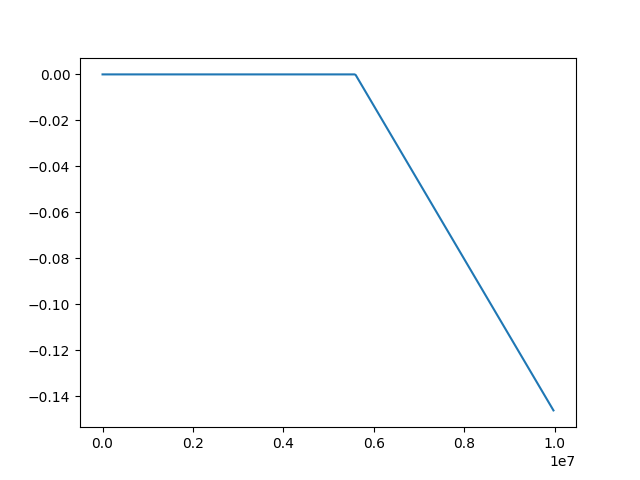
\includegraphics[width=.7\linewidth]{img/plot_1.png}
	\caption{Wykres błędu względnego od iteracji sumy dla v = (0.25+0.125)/2}
\end{figure}
	Jak widzimy błąd na początku jest bliski zeru a następnie rośnie na moduł liniowo.
	Najprawdopodobniej jest to spowodowane, że od pewnej iteracji suma jest na tyle duża w porównaniu do składnika, że przy dodawaniu ucinane są mało znaczące bity po tym jak wyrównane zostaną wykładniki.
\begin{itemize}
	\item	Zaimplementuj rekurencyjny algorytm sumowania.
	\item Wyznacz bezwzględny i względny błąd obliczeń. Dlaczego błąd względny znacznie zmalał?
	\item Porównaj czas działania obu algorytmów dla tych samych danych wejściowych.
	
	
\end{itemize}

Kod programu:

\begin{minted}{Python}
	float recsum(float* tab, int start, int end){
		if(start == end) return tab[start];
		int mid = start + (end-start)/2;
		return recsum(tab, start, mid) + recsum(tab, mid+1, end);
	}
\end{minted}

Dla danych wejściowych jak wyżej otrzymujemy:
\begin{lstlisting}
	
	Normal adding time elapsed: 0.035277 ===========
	SUM/ERROR/RERROR  2150474.5 -275474.5 -0.146919733333
	
	Recursive adding time elapsed: 0.088499 ===========
	SUM/ERROR/RERROR  1875000 0 0
\end{lstlisting}

Jak widzimy dodawanie rekurencyje zwraca dokładny wynik kosztem ponad 2x dłuższego czasu wykonania. Sumując rekurencyjnie zawsze dodajemy liczby porównywalnych rzędów wielkości co rozwiązuje wcześniejszy problem.

\begin{itemize}
	\item Przedstaw przykładowe dane wejściowe, dla których algorytm sumowania rekurencyjnego zwraca niezerowy błąd.
\end{itemize}

Dla v = 0.503940 program zwraca:

\begin{lstlisting}
Recursive adding time elapsed: 0.089134 ===========
SUM/ERROR/RERROR  5039399.5 0.500000000931 9.9218161077e-08
\end{lstlisting}


\section{Algorytm Kahana w języku C:}

Kod:

\begin{minted}{C++}
	float kahanSum(float* tab, int len) {
		float sum = tab[0];
		float compensate = 0.0;
		float tmp, buf;
		for(int i = 1; i < len; i++){
			tmp = tab[i] - compensate;
			buf = sum + tmp;
			compensate = (buf - sum) - tmp;
			sum = buf;
		}
		return sum;
	}
\end{minted}

Działanie programu opiera się na zachowywaniu młodszych bitów przy sumowaniu i dodawaniu ich do składnika sumy przy następnym dodawaniu.

Dla v = 0.503940:

\begin{lstlisting}
	Normal adding time elapsed: 0.035688 ===========
	SUM/ERROR/RERROR  5001516.5 37883.5 0.00751746239632

	Recursive adding time elapsed: 0.089134 ===========
	SUM/ERROR/RERROR  5039399.5 0.500000000931 9.9218161077e-08

	Kahan adding time elapsed: 0.104306 ===========
	SUM/ERROR/RERROR  5039400 9.31322574615e-10 1.84808226101e-16
\end{lstlisting}
	


\clearpage
\newpage

Cały kod używany w zadaniu 3 i 4:

\begin{minted}{C++}
#include<iostream>
#include<iomanip>
#include<ctime>
#define e7 10000000
//#define C (0.25+0.125)/2
#define C 0.503940

using namespace std;

float recsum(float* tab, int start, int end);
float normal_sum();
float kahanSum(float* tab, int len) {
	float sum = tab[0];
	float compensate = 0.0;
	float tmp, buf;
	for(int i = 1; i < len; i++){
		tmp = tab[i] - compensate;
		buf = sum + tmp;
		compensate = (buf - sum) - tmp;
		sum = buf;
	}
	return sum;
}


float *tab;
int main(){
	cout << setprecision(12);
	clock_t start, end;

	tab = new float[e7];
	for(int i = 0; i < e7; i++) tab[i] = C;

	start = clock();
	float sum = normal_sum();
	end = clock();
	cout << "\nNormal adding time elapsed: " << (end-start)*1.0/CLOCKS_PER_SEC << " ===========";
	cout << "\nSUM/ERROR/RERROR  " <<sum<<" "<< (e7*C - sum) <<" " << (e7*C - sum)/(C*e7) <<  endl;


	start = clock();
	sum = recsum(tab,0, e7-1);
	end = clock();
	cout << "\nRecursive adding time elapsed: " << (end-start)*1.0/CLOCKS_PER_SEC << " ===========";
	cout << "\nSUM/ERROR/RERROR  " <<sum<<" "<< (e7*C - sum) <<" " << (e7*C - sum)/(C*e7) <<  endl;


	start = clock();
	sum = kahanSum(tab, e7);
	end = clock();
	cout << "\nKahan adding time elapsed: " << (end-start)*1.0/CLOCKS_PER_SEC << " ===========";
	cout << "\nSUM/ERROR/RERROR  " <<sum<<" "<< (e7*C - sum) <<" " << (e7*C - sum)/(C*e7) <<  endl;

}

float normal_sum(){

	float sum = 0;

	for(int i = 0; i < e7; i++){
		sum += tab[i];
		if(i % 25000 == 0){

		// cout << i<< ": " << (i*C - sum) << endl;
		cout <<sum<<" "<< (i*C - sum) <<" " << (i*C - sum)/(C*e7) <<  endl;
		}
	} 
	cout << "#DATA_END\n";
	return sum;
}

float recsum(float* tab, int start, int end){
	if(start == end) return tab[start];
	int mid = start + (end-start)/2;
	return recsum(tab, start, mid) + recsum(tab, mid+1, end);
}
\end{minted}



\clearpage
\newpage

\section{Napisz program w języku C, który wyznaczy K najmniejszych liczb ze zbioru N elementowej nieposortowanej tablicy liczb typu float bazując na idei sortowania kubełkowego i algorytmie zaprezentowanym i wytłumaczonym na zajęciach na tablicy. Dokonaj analizy poprawności działania algorytmu i czasu wykonania dla innego algorytmu wyszukującego k K najmniejszych liczb dla zbioru liczb wygenerowanych w zakresach: $<0.0,0.3>$ i $<0.0, 3.0>$.
}

Kod programu:

\begin{minted}{C++}
#include <iostream>
#include <vector>
#include <cmath>
#include <list>
#include <ctime>

#define MAXVAL 1.0f
#define MINVAL 0.0f

using namespace std;



float max(const list<float> tab){
	float buff = tab.front();
	for(auto i = tab.begin(); i != tab.end(); ++i){
		if(*i > buff) buff = *i;
	}
	return buff;
}


float min(const list<float> tab){
	float buff = tab.front();
	for(auto i = tab.begin(); i != tab.end(); ++i){
		if(*i < buff) buff = *i;
	}
	return buff;
}

float max(float a, float b){
	return a>b ? a : b;
}

list<float> k_mins( const list<float> workingTab, int k, int n_buck){
	list<float> result;
	if(k == 0) return result;
	//cout << 'D' << flush;
	
	float minim = min(workingTab);
	float maxim = max(workingTab);

	float min1 = 0;
	float max1= maxim - minim;

	vector<list<float>> buckets;
	buckets.resize(n_buck);


	for(auto tabElem = workingTab.begin(); tabElem != workingTab.end(); ++tabElem){
		buckets[floor(
			min((float)(n_buck-1), //min dlatego żeby 
			//maksymalna wartość nie trafiła do kubełka o numerze n_buck  
				max(n_buck+log2(*tabElem-minim), //wszystkie 
				//watrości mniejsze niż 2^(n_buck) do zerowego
				0.0f)))].push_back(*tabElem);
	}


	//cout << "=========== POTRZEBUJE JESZCZE " << k <<" liczb ================\n";
	for(int i = 0; i < buckets.size(); i++){
		//   cout << "W kubelku nr " << i << " jest " << buckets[i].size() << "liczb" << endl; 
		if(result.size() + buckets[i].size() <= k){
			result.merge(buckets[i]);
		}
		else{
			result.merge(k_mins(buckets[i], k - result.size(), n_buck));
			break;
		}
	}
	return result;
}

list<float> classic_k_mins(list<float> workingTab, int k){
	workingTab.sort();
	list<float> res;
	int it = 0;
	for(auto i = workingTab.begin(); i != workingTab.end() && it < k; ++i){
		res.push_back(*i);
		it++;
	}
	return res;
}


int main(){
	srand(time(NULL));
	list<float> test = {2.5, 34, 5.3, 34.5, .43, 5.4, 2, 123094, 542, 0.0432423, 0.0432434};
	list<float> test2;
	const float LIM = 0.3;
	const int K = 10;



	clock_t start, end;
	list<float> res;

	for(int N = 100; N <= 10000000; N*=10){
		test2.clear();
		cout << "\n\nTesting 10 min of " << N << " numbers\n";

		for(int i = 0; i < N; i++){
			test2.push_back(static_cast <float> (rand()) / (static_cast <float> (RAND_MAX/LIM)));
		}

		start = clock();
		res = k_mins(test2, K, 256);
		end = clock();
		res.sort();

		cout << "\nExercise version time elapsed: " 
		<< (end-start)*1.0/CLOCKS_PER_SEC << " ===========\n";
		for(auto i = res.begin(); i != res.end(); ++i) cout << *i << " ";

		start = clock();
		res = classic_k_mins(test2, K);
		end = clock();
		cout << "\nNormal version time elapsed: " 
		<< (end-start)*1.0/CLOCKS_PER_SEC << " ===========\n";
		res.sort();
		for(auto i = res.begin(); i != res.end(); ++i) cout << *i << " ";
		cout << endl;
	}
	return 0;
}
\end{minted}

Przeprowadzono testy polegające na znajdywaniu 10 najmniejszych liczb spośród 100, 1000, ..., 10000000 losowych.
Ich wyniki poniżej.

Dla przedziału $[0, 0.3]$
\lstinputlisting{test0.3.txt}


Dla przedziału $[0, 3]$
\lstinputlisting{test3.txt}